\chapter{DETs Selection Framework}
\label{cha:3_framework}
This chapter describes the structure of the framework, identifies the stakeholders involved and their roles, and defines the assessment methodology and sustainability dimensions along with their respective indicators. A summary table is provided for each dimension, while the complete table can be found in Appendix \ref{cha:attachment_overleaf_comparison}.

Section \ref{sec:3.1_framework_structure} introduces the framework describing its structure. Section \ref{sec:3.2_stakeholders} describes the stakeholders involved and provides a high-level schema, while Section \ref{sec:3.3_assessment} defines the assessment methodology. Finally, Section \ref{sec:3.4_sustainability_dimensions} defines the sustainability dimensions and their indicators.

\section{Introduction to the framework}
\label{sec:3.1_framework_structure}
In recent years, the continuous integration of software and hardware solutions into learning, teaching, and administrative activities has led to the problem of selecting digital education technologies. As discussed in the previous chapters, this process seems to take place with little to no consideration of sustainability, while economic factors remain the dominant driving force. Recent studies have highlighted that the absence of evaluation criteria, along with common challenges such as limited financial resources, significantly impacts the procurement of sustainable digital education technologies \cite{huang_building_2023-1}. In addition, research literature concurs on the multi-dimensional nature of sustainability and its impact on the long-term viability and effectiveness. The purpose of the framework is to address this gap by providing a structured approach to evaluating whether DETs meet the sustainability requirements of higher education settings. The model is designed to assist decision makers in making informed choices that balance trade-offs across all the involved dimensions. \\
%As shown in the figure (insert figure), the framework consists of:
The framework consists of:
\begin{itemize}[noitemsep, topsep=4pt, parsep=0pt, partopsep=0pt]
    \item A set of stakeholders with distinct roles
    \item A set of interrelated dimensions, each assessed through a set of indicators
    \item Distinct sets of indicators (one per dimension), each associated with specific metrics and assessment methods
\end{itemize}
%Due to the wide range of digital technologies - both hardware and software - that could be assessed by this framework, it allows a versatile approach where some indicators could be re-assessed in a different dimension than the starting one, at the discretion of who is in charge of the selection process. Furthermore, some indicators may fit better to certain circumstances and the freedom to exclude some indicators is granted if the application is particularly complex or not possible at all.
Given the wide range of digital technologies, both hardware and software, that this framework can assess, it offers a versatile approach. Certain indicators may be reassessed under a different dimension instead of their initial one, at the discretion of those responsible for the selection process. Furthermore, some indicators may be more suitable for specific circumstances, and the flexibility to exclude certain indicators is granted when their application is particularly complex, counterproductive, or not possible at all. Examples of digital education technologies are listed in Table \ref{tab:examples_DETs}, grouped by category.

Each component of the framework will be further discussed in its respective section.

\begin{table}[ht!]
    \centering
    % \small
    \scriptsize
    % \tiny
    % \footnotesize
    \renewcommand{\arraystretch}{1.5} % Adjust row height
    \begin{tabular}{|>{\centering\arraybackslash}m{6.5cm}|>{\centering\arraybackslash}m{5.5cm}|}
        \hline
        \textbf{Category} & \textbf{Education technology} \\
        \hline
        \multirow{3}{*}{Cloud computing and virtual machines} & Amazon AWS  \\
        \cline{2-2}
        & Azure \\
        \cline{2-2}
        & Heroku \\
        \hline
        \multirow{3}{*}{Communication} & Discord  \\
        \cline{2-2}
        & Slack \\
        \cline{2-2}
        & Skype \\
        \hline
        \multirow{3}{*}{Gamification and Quiz} & Kahoot! \\
        \cline{2-2}
        & Mentimeter \\
        \cline{2-2}
        & Socrative \\
        \hline
        \multirow{3}{*}{Generative AI} & ChatGPT  \\
        \cline{2-2}
        & PaperPal \\
        \cline{2-2}
        & Writefull \\
        \hline
        \multirow{4}{*}{Learning management systems} & Blackboard \\
        \cline{2-2}
        & Canvas \\
        \cline{2-2}
        & Google Classroom \\
        \cline{2-2}
        & Moodle \\
        \hline
        \multirow{2}{*}{Massive Open Online Courses (MOOCs)} & Learnn \\
        \cline{2-2}
        & Udemy \\
        \hline
        \multirow{2}{*}{Video streaming} & Kaltura \\
        \cline{2-2}
        & Youtube \\
        \hline
        \multirow{5}{*}{Video conferencing} & Big Blue Button (BBB) \\
        \cline{2-2}
        & Google Meet \\
        \cline{2-2}
        & Microsoft Teams \\
        \cline{2-2}
        & Webex \\
        \cline{2-2}
        & Zoom \\
        \hline
        \multirow{3}{*}{Writing} & Google Documents \\
        \cline{2-2}
        & Microsoft Word \\
        \cline{2-2}
        & Overleaf \\
        \hline

    \end{tabular}
    \caption{Categories of DETs considered in framework development and examples}
    \label{tab:examples_DETs}
\end{table}

%Three of the five dimensions—Economic, Social, and Environmental—are derived from the widely recognized three Pillars of Sustainability concept, ensuring alignment with fundamental sustainability principles. These dimensions capture the financial feasibility, societal impact, and ecological footprint of DETs, respectively. The Pedagogical dimension is adapted from previous research in educational technology sustainability, recognizing the critical role of digital tools in supporting learning effectiveness and teaching methodologies.  Each dimension is assessed through a set of carefully selected indicators, which provide measurable criteria for evaluation. These indicators, in turn, are associated with specific metrics and assessment methods to ensure a structured and objective evaluation process. 

\section{Stakeholders}
\label{sec:3.2_stakeholders}
The stakeholders taking part in the dynamics of the framework are the following:
\begin{itemize}[noitemsep, topsep=4pt, parsep=0pt, partopsep=0pt]
    \item \textbf{Student and teachers} - Students and teachers, but also researchers, employees, and anyone who makes use of DETs and services offered by the university.
    \item \textbf{Provider} - The vendor or organization that offers its products to the university. It is expected to act as the service provider or as the cloud provider.
    \item \textbf{University} - IT specialists, IT heads, and all those who represent the institution and contribute to the DETs selection process.
\end{itemize}
\noindent

The high-level view of the framework illustrated in Figure \ref{fig:framework_stakeholders} describes how the stakeholders are involved in sustainability. The figure emphasizes how the university's control over many aspects of sustainability is reduced in the presence of an external provider. When dealing with FLOSS or self-hosting, higher education institutions assume the role of the provider, gaining stronger control over every dimension and limiting the impact of the provider.

% \begin{figure}[ht!]
%   \centering
%   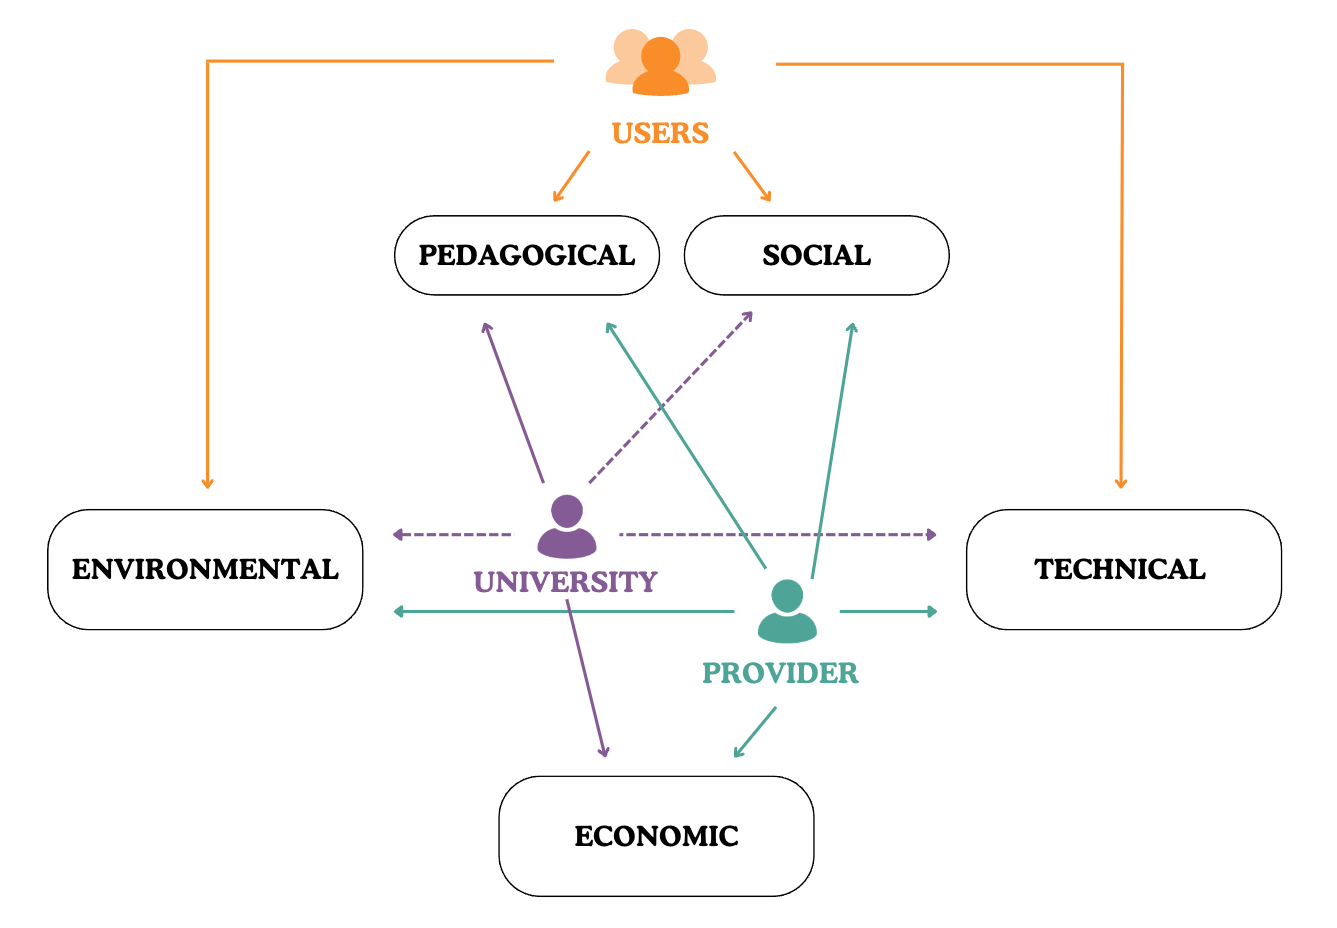
\includegraphics[width=0.85\textwidth]{img/framework_roles.png}
%   \caption{\centering{Actors and sustainability dimensions}}
%   \label{fig:framework_roles}
% \end{figure}

\begin{figure}[ht!]
  \centering
  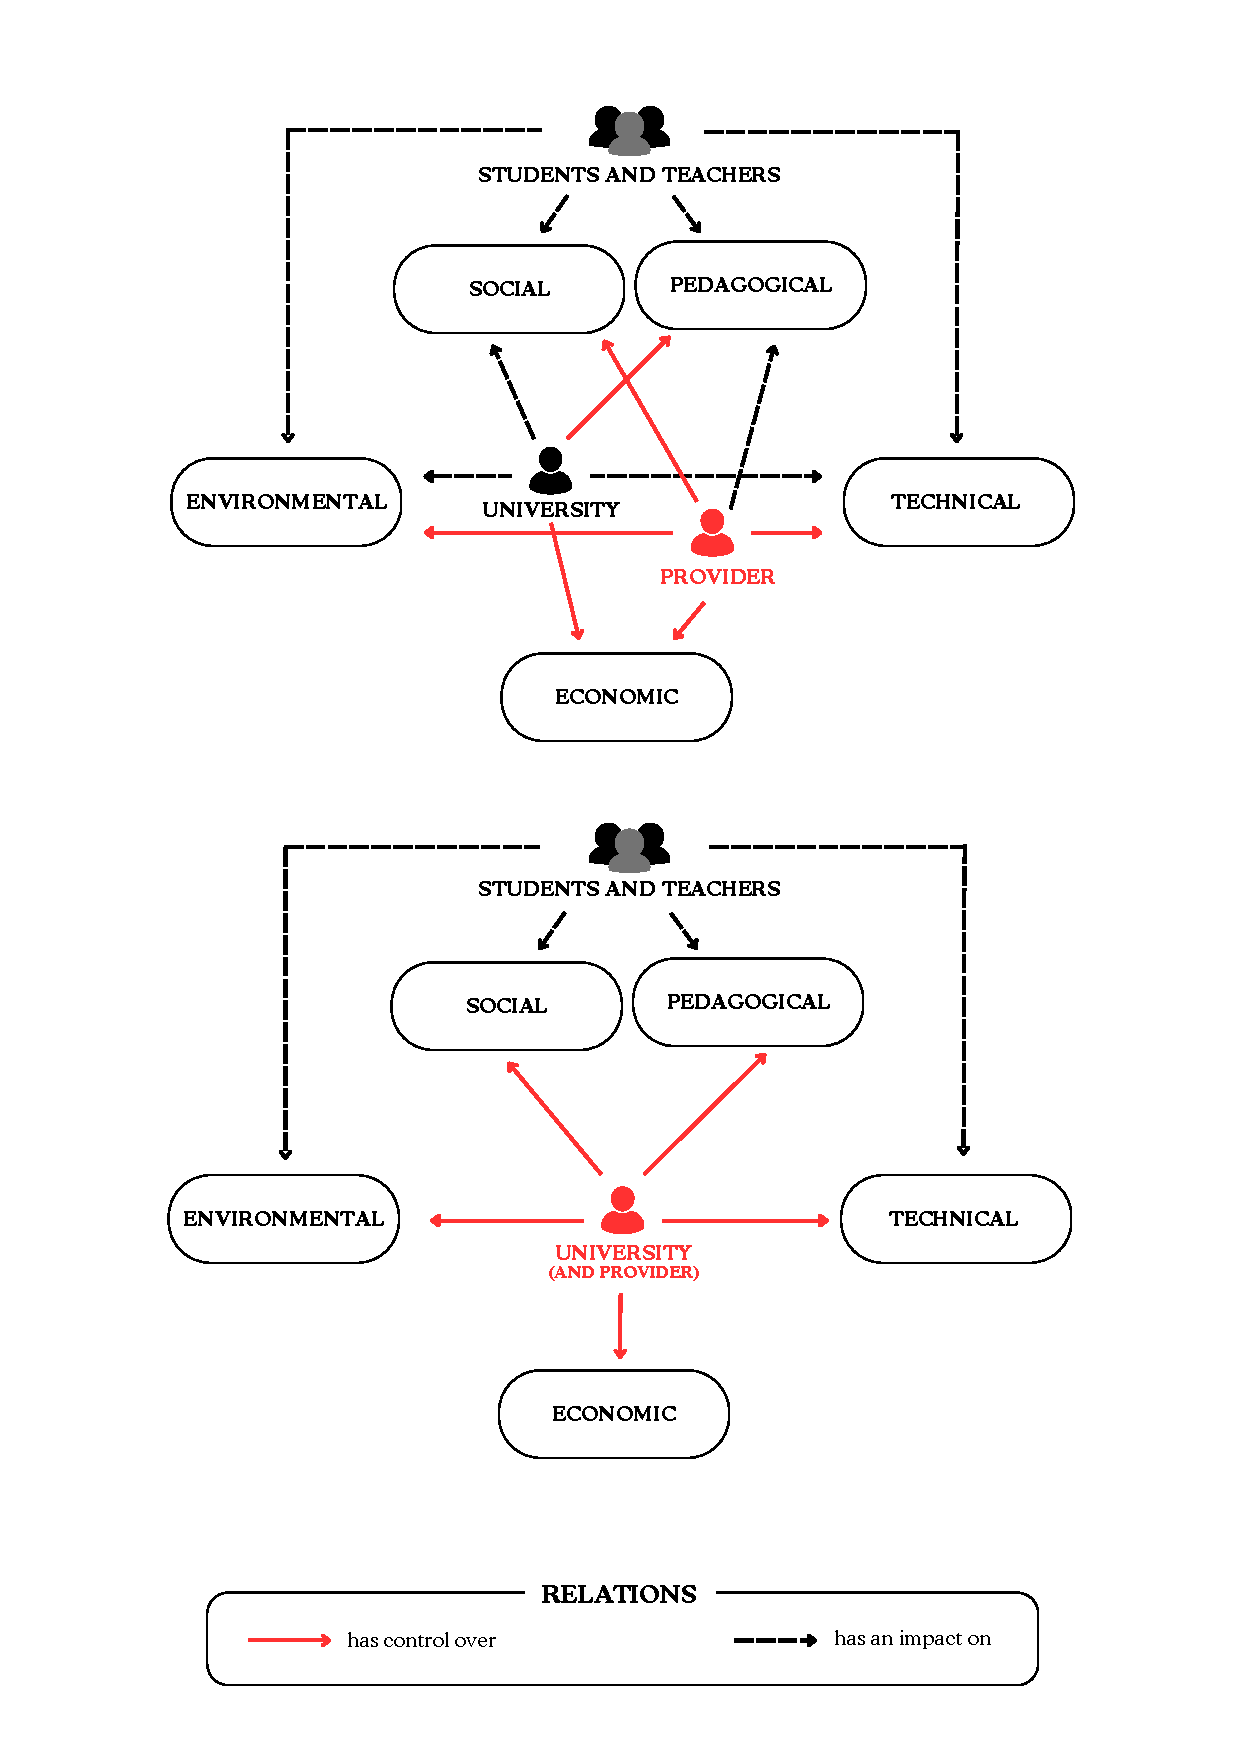
\includegraphics[width=0.95\textwidth]{attachments/framework_stakeholders.pdf}
  \caption{\centering{Relations between stakeholders and sustainability dimensions. The upper section illustrates these relations when the provider acts as the service provider, while the lower section shows them when the university assumes this role. }}
  \label{fig:framework_stakeholders}
\end{figure}
% Schema con controllo e impatti con due colori diversi
% Uno che mostra con provider e uno senza
% cambiare utenti con studenti e insegnanti

\section{Assessment methodology}
\label{sec:3.3_assessment}
To systematically assess the sustainability of digital education technologies, the framework employs a revised traffic-light rating system that categorizes each indicator into three levels: Red, Yellow, and Green. This choice is based on the idea that the traffic-light system provides an intuitive and immediate way to interpret the performance of each indicator. The meaning of the levels is defined as follows:
\begin{itemize}[noitemsep, topsep=4pt, parsep=0pt, partopsep=0pt]
    \item \textbf{Red light} - An indicator is classified as red when the technology under consideration does not meet the minimum requirement.
    \item \textbf{Yellow light} - A yellow light is assigned when the DET meets a minimum acceptable threshold for the indicator examined. This classification highlights the need for significant improvement, but it can also represent a situation of uncertainty in which further investigation is required.
    \item \textbf{Green light} - A green light confirms that the assessed DET is fully aligned with the indicator's requirement.
\end{itemize}

For comparative analysis between different DETs or multiple versions of the same DET, the results are numerically converted into a scoring system, where \textbf{red} equals -1, \textbf{yellow} equal 0, and \textbf{green} equals 1. The total score serves as a comparative metric, facilitating the ranking of different solutions based on their overall sustainability performance. However, when assessing an education technology without comparable alternatives or when evaluating the adoption of a new DET, the total score may lack contextual significance. In such cases, the overall distribution of traffic-light indicators provides a clearer qualitative evaluation, highlighting areas of strength and potential improvement without reducing the assessment to a single numerical value. Clearly, if a dimension lacks green lights or if the majority of the indicators turn red, the adoption of the technology is highly discouraged.


\section{Sustainability dimensions}
\label{sec:3.4_sustainability_dimensions}
The framework is built upon a multi-dimensional approach that integrates established sustainability principles with domain-specific considerations, i.e., pedagogical in the context of education and technical in the context of digital technologies. The first set of dimensions - economic, social, and environmental - are derived from the widely recognized three pillars of sustainability model, ensuring alignment with fundamental sustainability principles. The pedagogical dimension is adapted from previous research in sustainable education and a critical analysis of digitalization. Finally, the technical dimension is derived from the software-specific sustainability frameworks developed by Lago et al. \cite{lago_framing_2015} and Andrikopoulos et al. \cite{andrikopoulos_software_2021}, with modifications to accommodate broader technological solutions such as those of edtech. 

The following sections detail each dimension, its relevance, and the indicators used for assessment.

\subsection{Economic dimension}
The economic dimension represents the economic feasibility of a technology used in the context of higher education throughout its entire lifecycle. Budgetary and financial constraints exert a strong influence over the selection process, determining cost efficiency as a central theme.
This perspective builds upon the sustainability-aware framework proposed by Andrikopoulos et al. \cite{andrikopoulos_software_2021}, which defines economic sustainability in Software as a Service (SaaS) by emphasizing the maximization of return of expenses. However, since this model was specifically designed for SaaS, it requires adaptation when applied to a wider range of digital education technologies.
From Andrikopoulos’ framework, we can derive return of expanses as a fundamental indicator, as well as the related indicators of provisioning and scaling policies. By enhancing this aspect, cost efficiency is not only confined to expenditures reduction but also encompasses the optimization of resource allocation to ensure sustainability.
Furthermore, following the insights of Fiebig et al. \cite{fiebig_heads_2023} and Angeli et al. \cite{angeli_conceptualising_2022}, it is crucial to account for the economic implications of discontinuing a technology or migrating to alternative ones, confirming the need for indicators that examine exit costs and the influence of vendor synergies (i.e. lock-in). These factors can significantly impact the institution's ability to transition between different solutions and must be considered in the selection process.
This set of indicators is designed to prioritize the long-term economic viability of a technology over its short-term cost benefits.

\subsubsection{Return of Expenses}
The concept of return of expenses (RoE) can be defined as the degree of efficiency in consuming resources, such as cloud, hardware, and monetary assets, with respect to the generated revenue \cite{andrikopoulos_software_2021}.
During the selection process, universities may encounter two different scenarios:
\begin{enumerate}[noitemsep, topsep=4pt, parsep=0pt, partopsep=0pt]
    \item The technology is already in use, served on-premise or through an external provider, and there is an intention to migrate towards an alternative.
    \item The technology has not yet been adopted.
\end{enumerate}
In the first case, RoE serves to estimate the degree of success and the economic benefits that would result from migrating the existing technology to an alternative solution.
In the second case, the institution must define what constitutes "generated revenue" within its domain and establish an acceptable threshold. For example, this indicator should help answer the following questions:
\begin{center}
    \textit{“How likely is the DET to be adopted by users?”} \\
    \textit{"How likely is the DET to remain in use over time?"}
\end{center}
When applied to software solutions, this indicator is particularly useful in cases such as comparing cloud-based tools with technologies available exclusively on-premises. Furthermore, if RoE is used to compare different deployment models of the same technology, the generated revenue may be similar across cases and can therefore be excluded from the evaluation process. However, RoE is inherently limited by the vast range of technologies it can assess, necessitating a more specific definition tailored to each case. Developing systematic evaluation methods to estimate return of expenses remains an open area for future research. The exclusion of this indicator from the study was not considered, as even a high-level analysis can provide valuable insights for its assessment.

\subsubsection{Provisioning}
The provisioning indicator aims to measure the resources allocated, either cloud-based or local, in relation to the expected resources required to ensure the proper operation of the service. Despite its technical nature, the provisioning indicator is placed within the economic dimension as it directly impacts cost-efficiency. In fact, resources represent a significant cost factor that cannot be ignored, and minimizing energy waste and underutilized resources is essential to reduce costs. Typically, an incorrect estimation of the required resources leads to two possible outcomes: over-provisioning and under-provision. Over-provisioning leads to unnecessary expenses due to unused resources, while under-provisioning leads to performance degradation and potential loss of generated value (i.e. university community cannot make use of the technology).
This indicator is evaluated through the Quality of Provisioning metric, defined as:
\[
\text{Quality of Provisioning (QoP)} = \frac{\text{Allocated Resources}}{\text{Used Resources}}
\]
The QoP indicator is designed to facilitate the comparison of different deployment models, generating measures for many provisioning cases that are later correlated with the cost of the allocated resources. The result is the expected cost per user. It is evident that when comparing local infrastructure with cloud-based solutions, the indicator tends to favor cloud resources. This is because cloud providers distribute costs across the user base, leading to optimized resource allocation that is hardly achievable in other contexts. Additionally, in the case of cloud-based solutions, detailed information about provisioning is often not disclosed, as resources are abstracted and offered at a fixed price rather than being transparently allocated based on actual usage.

This indicator can also be later reiterated in the context of technical sustainability.

\subsubsection{Scaling policies}
The scaling policies indicator integrates the provisioning indicator by examining how resources are managed once provisioned. While provisioning assesses the efficiency of resource allocation, scaling policies analyze how these resources are adjusted over time.
Except in special cases, the on-demand approach is preferred over the always-on model, which tends to generate more waste. Ideally, the system should always be able to compensate for the load. The effectiveness of the indicator is bound to the technical characteristics of the technology, as different architectures and infrastructures impose varying constraints and possibilities for resource scaling. This indicator is evaluated through the same metric as the previous one, which should be reiterated according to the scaling policy to reflect the related costs. Alternatively, the average percentage of wasted resources (\%) could provide valuable insights.

\subsubsection{Vendor synergies (lock-in)}
Vendor synergies refer to the advantages and operational efficiencies that emerge when universities integrate multiple digital services and infrastructures from a single vendor. Cloud providers often offer bundled services with advantageous pricing models, which are highly integrated into the vendor ecosystem. These practices often lead to reduced management complexity and potentially lower costs, but they may also enable lock-in mechanism and increased dependence on proprietary standards and services \cite{komljenovic_rise_2021}\cite{fiebig_heads_2023}. For example, Google Workspace and Microsoft 365 are highly integrated platforms that provide several solutions within the same ecosystem. Even if universities host services on their own digital infrastructure, they may still rely on proprietary standards and integrations, making it difficult to migrate to alternative solutions without significant costs and effort.
This indicator aims to identify and quantify vendor synergies that may impact the migration process away from the vendor’s ecosystem. To develop a metric, the institution should analyze the technology to identify evidence of lock-in and soft lock-in practices. An acceptable level is when the impact of synergies is manageable during the migration process, while soft lock-in can be neglected if its influence is minimal\footnote{In this study, soft lock-in refers to all the features and characteristics that enhance the technology without imposing legal or technical restrictions.}.

\subsubsection{Exit costs}
The purpose of the exit cost indicator is to quantify the effort, and thus the cost, of moving either toward an external provider or to the university's digital infrastructure. In the first case, the total cost of the migration consists of the expense of IT staffing and the price agreed with the new vendor. In the second case, other complexities come into play, such as the cost of upgrading the internal infrastructure (both hardware and software components) and the procurement of new technical staff.       

\bigskip

\begin{table}[ht!]
    \centering
    \small
    % \scriptsize
    % \tiny
    % \footnotesize
    \renewcommand{\arraystretch}{1.5} % Adjust row height
    \begin{tabular}{|>{\centering\arraybackslash}m{3cm}|>{\centering\arraybackslash}m{3.1cm}|>{\centering\arraybackslash}m{2.9cm}|>{\centering\arraybackslash}m{2.9cm}|>{\centering\arraybackslash}m{2.9cm}|}
        \hline
        \textbf{Indicator} & \textbf{Metric} & \textbf{Red light} & \textbf{Yellow light} & \textbf{Green light} \\
        \hline
        Return of Expenses & To be defined within the institution & Low or absent generated value & Acceptable generated value & Optimal generated value \\
        \hline
        Provisioning & Quality of Provisioning & High cost per user & Acceptable cost per user & Low cost per user \\
        \hline
        Scaling policies & Waste of resources & High waste & Acceptable waste & Low waste \\
        \hline
        Vendor synergies & Vendor make use of lock-in practices & Legal/technical restrictions, proprietary standards, etc. & Soft lock-in & Negligible or no soft lock \\
        \hline
        Exit costs & Total expenses of exit/migration & High costs & Acceptable costs & Very low costs \\
        \hline
    \end{tabular}
    \caption{Summary of the economic indicators}
    \label{tab:summary_economic_indicators}
\end{table}

\subsection{Technical dimension}
Technical sustainability is the dimension that requires software and hardware systems to remain operational, efficient, and adaptable over time. This dimension lays its foundations on key principles derived from distributed systems theory, such as dependability and maintainability \cite{tanenbaum_distributed_2006}. In this framework, the concept of dependability is not treated as a mere technical definition, but is integrated with the concept of Quality of Service (QoS) presented by Andrikopoulos et al. \cite{andrikopoulos_software_2021}. QoS relates to how users perceive the system and its ability to fulfill their expectations, while dependability refers to the system's ability to deliver its functionality in depth of time. QoS relies on dependability, incorporating its operational and architectural aspects, like availability, reliability, and scalability, which are reshaped according to users' need. Maintainability, on the other hand, remains faithful to its classical definition, requiring ease and efficiency in updating, upgrading, and repairing the system. These two principles intersect in the operational indicator of adaptability, which is essential for the long-term viability of the system. Typically, private companies withhold their system specifications from the public. Thus, when dealing with external providers who are not likely to share such information, the assessment of technical sustainability is limited to a high-level perspective.    

\subsubsection{Availability}
In the context of the tech business, availability is often defined as "the ability to be operational at all times, from anywhere, using any device"\footnote{Lucidchart - \href{https://www.lucidchart.com/blog/reliability-availability-in-cloud-computing}{https://www.lucidchart.com}}. Although this definition applies to web technologies, it suffers the influence of the cloud computing model. In the wider context of education technologies, a more appropriate definition is "the ability to be operational at a given time"\footnote{Atlassian - \href{https://www.atlassian.com/incident-management/kpis/reliability-vs-availability}{https://www.atlassian.com}}. This implies that, depending on the DET, it is not required to be always available, but rather to be available when needed. For example, a video conferencing tool used exclusively to host lectures has no reason to be available before and after the class schedule. Typically, high availability is required for critical services and systems, such as administrative tools and email services. This indicator is evaluated through the availability percentage metric (also known as uptime percentage), defined as:
\[
    \text{Availability percentage} = \frac{\text{Uptime}}{\text{Total time}} \times 100
\]
Clearly, this metric may be difficult to estimate during the selection process, but for DETs already provided as a service, availability measurements can be conducted based on historical performance data. An acceptable level of availability should be defined based on the specific DET under evaluation.

\subsubsection{Reliability}
Similarly to the previous indicator, reliability is defined as "the probability that a system or component will perform its intended function without failure under specified conditions for a given period". This implies that although a certain DET is available, it is not necessarily reliable. 

Different metrics have been developed to assess reliability. One of the most popular is the error rate metric, expressed as a percentage:
\[
    \text{Error rate} = \frac{\text{Number of failed operations}}{\text{Total number of operations}} \times 100
\]
Like availability, high reliability is required for critical services and systems, such as remote proctoring software or learning management systems with assessment features.

\subsubsection{Scalability}
As defined in distributed systems theory, the scalability of a system refers to its ability to increase or decrease its scale in terms of size, geographic distribution, and administrative span \cite{tanenbaum_distributed_2006}. In this framework, the focus is on size, since it determines how likely a technology is to accommodate new users, data, and resources. Among the dependability attributes, scalability represents the most difficult to examine, as cloud providers typically abstract the underlying system from users. To evaluate scalability, two cases can be distinguished:
\begin{itemize}[noitemsep, topsep=4pt, parsep=0pt, partopsep=0pt]
    \item DET is offered by a vendor - The indicator is generally not applicable, since the complexity is delegated to the external provider. However, for cloud-based solutions, monitoring metrics can offer useful insights, such as average response time.
    \item DET is deployed as self-hosted - The study of the technology should determine whether it sufficiently supports scalability techniques.
\end{itemize}
For example, if a DET does not support either horizontal or vertical scaling, the indicator will result in a red light. Conversely, if a DET supports load balancing, as well as both vertical and horizontal scaling, the indicator will result in a green light.

\subsubsection{Maintainability}
Maintainability is a key principle in the context of systems and software architectures. It can be seen as a set of fundamental properties, such as availability, upgradability, and repairability\footnote{Microsoft page on GitHub - \href{https://microsoft.github.io/code-with-engineering-playbook/non-functional-requirements/maintainability/}{https://microsoft.github.io/code-with-engineering-playbook/}}. Given their significance, each of these properties give rise to an indicator. In this framework, maintainability is confined to the ability of a software or a system to be easily configured, updated, and upgraded. In addition to the installation and distribution methods, the quality of the documentation and support plays a crucial role in achieving a satisfactory level of maintainability. To obtain a good score, ease and efficiency in installing and updating the software are required.

\subsubsection{Adaptability}
The concept of adaptability varies depending on the subject: software architectures and system architecture. The former is built upon extensibility, flexibility, tunability, and fixability \cite{fayad_aspects_1996} and refers to the willingness of software architectures to accept changes without significant code rewrites or architecture redesign. Adaptable software is likely to support new features and changes without extensive rework, allow integration of new and external components, and facilitate migration to other systems. The latter refers to the capability of a system to manage changes in hardware and software components while continuing to fulfill its requirements \cite{tanenbaum_distributed_2006}. Adaptable systems promote modularity and support the integration of new hardware and software technologies.

Research literature suggests some metrics for this indicator, such as those proposed by Subramanian et al. at the University of Texas at Dallas \cite{subramanian_metrics_2001}. However, the assessment requires in-depth knowledge of the software architecture or system architecture and inevitably becomes more complicated when external solutions are adopted. In this study, the adaptability indicator is limited to verifying how a given solution integrates within the institution's infrastructure (e.g., Single Sign-On) and how it interacts with third-party services. To obtain a green light, integration with both is mandatory.  

\subsubsection{Repairability}
Software repairability (or fixability) is a multifaceted attribute, generally considered a subset of maintainability. It is defined as the ability to resolve defects without introducing unintended issues elsewhere. From a broader perspective, software repairability is not limited to fixing bugs and inaccuracies in the code, but also includes addressing errors and malfunctions that affect functionality. The disruption of a cloud service is not necessarily related to a software issue. Factors such as connectivity problems or underlying infrastructure failures can also be responsible. Therefore, software repairability refers to interventions within the software itself, either through code modifications or control tools, and to related components that may contribute to malfunctions, ensuring the recovery of availability and reliability when they are compromised.

The repairability indicator, when applied to software, results in a green light when both code changes (i.e., open-source) and direct intervention on operational factors are permitted. It results in a yellow light when code modifications are not allowed, but it is still possible to take actions on related factors. Finally, it results in a red light when no repair interventions are possible.

The definition of hardware repairability, instead, is inspired by the French Repairability Index, which aims to assign a score that quantifies the ease of repair for electrical and electronic devices\footnote{French Repairability Index - \href{https://repair.eu/it/news/the-french-repair-index-challenges-and-opportunities/}{https://repair.eu/}}. To be classified as repairable, hardware should be accompanied by repair manuals and guidelines and should be designed for simple assembly and disassembly. Additionally, spare parts should be available, easy to find, and reasonably priced. Finally, another factor that ensures better repairability is the absence of artificial barriers, such as soldered components.

The repairability indicator, when applied to hardware components, provides a score that ranges from 1 to 5, where 1 indicates poor repairability and 5 indicates high repairability.

\bigskip

\begin{table}[ht!]
    \centering
    \small
    % \scriptsize
    % \tiny
    % \footnotesize
    \renewcommand{\arraystretch}{1.5} % Adjust row height
    \begin{tabular}{|>{\centering\arraybackslash}m{3cm}|>{\centering\arraybackslash}m{3.1cm}|>{\centering\arraybackslash}m{2.9cm}|>{\centering\arraybackslash}m{2.9cm}|>{\centering\arraybackslash}m{2.9cm}|}
        \hline
        \textbf{Indicator} & \textbf{Metric} & \textbf{Red light} & \textbf{Yellow light} & \textbf{Green light} \\
        \hline
        Availability & Uptime (\%) & \multicolumn{3}{c|}{To be defined based on the DET} \\ 
        \hline
        Reliability & Error rate (\%) & \multicolumn{3}{c|}{To be defined based on the DET}  \\
        \hline
        Scalability & Scalability support & Little to no support for scalability techniques & Partial support for scalability techniques, with limitations in the long-term & Support scalability techniques \\
        \hline
        Adaptability & Degree of integration within university infrastructure and third-party components & No integration & Partial integration (e.g., only SSO) & Full integration (university infrastructure and multiple third-party components) \\
        \hline
        Maintainability & Ease of configuration, updates, and upgrades & Difficult to configure/update; poor documentation and support & Moderate ease of installation and updates; limited documentation and support & Easy and efficient installation, configuration, and updates; comprehensive documentation and support \\
        \hline
        \multirow{2}{*}{Repairability} & Interventions allowed & No interventions allowed & Limited interventions allowed (e.g., only infrastructure)  & Full interventions allowed (code and infrastructure) \\
        \cline{2-5}
         & Ease of hardware repair (availability of manuals, ease of disassemble, availability of spare parts, price of spare parts, and artificial barriers) & Score: 1–2 (poor repairability) & Score: 3 (moderate repairability) & Score: 4–5 (high repairability) \\
        \hline
    \end{tabular}
    \caption{Overview of technical indicators}
    \label{tab:overview_technical_indicators}
\end{table}

\newpage % ATTENTION

\subsection{Social dimension}
Social sustainability is the dimension that fosters accessibility, inclusion, equity, and social interaction. Education technologies have the potential to achieve equal access to education for all, as well as to promote social well-being and reduce costs \cite{haleem_understanding_2022}. During the pandemic, the hasty introduction of digital tools without considering learners' nneds led to the marginalization of certain students due to unstable internet connections and a lack of access to digital devices \cite{haleem_understanding_2022}. Through social sustainability, institutions must ensure greater access to education, mitigating inequalities due to disabilities, low-income backgrounds, and geographical barriers. Additionally, as digital competencies become increasingly essential, institutions should also promote digital citizenship and the development of digital skills \cite{crick_covid-19_2021}.

The engagement of private companies in educational dynamics requires more effort to achieve social sustainability. A key aspect is the privacy risk related to the unchecked collection and use of sensitive data and learning analytics\cite{komljenovic_rise_2021}. Universities should safeguard the privacy of users, preventing the exploitation of student and faculty data for commercial purposes. From a more technical perspective, Andrikopoulos et al. suggest that the level of awareness also plays an important role in this dimension\cite{andrikopoulos_software_2021}. Vendors and universities are required to actively participate in sustainability efforts and to keep their community (i.e., university members) aware of the changes and decisions that affect it.

Finally, institutions should favor solutions that positively impact their personnel and students. The outsourcing trend is leading to a reduction of internal knowledge and capability, while universities should promote innovation and collaboration and achieve greater autonomy.

\subsubsection{Community awareness}
Awareness of the community is a concept adapted from the framework proposed by Andrikopoulos et al.\cite{andrikopoulos_software_2021}. Their intuition is to keep the community in the loop about changes and decisions affecting the system. By increasing the rate of awareness about the system, particularly regarding sustainability-related decisions, the community can be actively engaged in the efforts to increase the system's sustainability. This indicator assesses whether the university or the external provider keeps the university members informed about changes and their subsequent sustainability implications. This practice has the potential to improve transparency and should not be reduced to a mere change-log, which would inevitably result in a red light. To obtain a green light, awareness efforts must be driven by sustainability objectives.

\subsubsection{Involvement in sustainability}
Involvement in sustainability, rather than technology, is related to its owner. This indicator quantifies the distance between the provider (i.e., the university or the vendor) and a sustainability claim or study. The underlying idea is that if a sustainability study is directly attributable to the provider, then it can be considered actively engaged in sustainability efforts. Conversely, if finding a sustainability claim requires tracing multiple relationships through a network, the provider’s involvement is indirect and potentially superficial. For example, if the provider has no sustainability claims, it is not actively engaged. If the provider is associated with at least one organization that is involved in sustainability, then its distance is one "hop". Otherwise, at least one more hop is required, and becomes too distant to be considered involved in sustainability.

\subsubsection{Inclusion}
Digital education technologies should guarantee equal access for all learners regardless of disabilities, socioeconomic status, and geographical constraints \cite{haleem_understanding_2022}. To assess the inclusiveness of education technologies, two key aspects of accessibility should be considered:
\begin{itemize}[noitemsep, topsep=4pt, parsep=0pt, partopsep=0pt]
    \item Technological accessibility - Focuses on hardware and software requirements necessary for effective use.
    \item Inclusive usability – Focuses on how the technology accommodates individuals with disabilities and diverse learning needs.
\end{itemize}

DETs are required to achieve technological accessibility by limiting technological barriers, particularly in terms of hardware and software requirements, that may preclude some individuals from using them. In the case of remote learning, required bandwidth and processing power should be minimized, while device compatibility should be guaranteed as much as possible. For example, Zoom typically regulates video quality based on the available bandwidth. However, this could lead to inefficiency and a degraded user experience for those with low bandwidth or outdated devices.

Technological accessibility is addressed within the environmental dimension, since many of its aspects, such as performance optimization, technical requirements, and bandwidth usage, are closely connected to environmental concerns. Optimization has the potential to reduce energy consumption, while lower technical requirements can ensure wider compatibility with older devices, thus contributing to the reduction of electronic waste. In addition, efficient bandwidth usage can mitigate the impact of data transmission, which is particularly relevant given the increasing energy demands of cloud computing \cite{angeli_conceptualising_2022}.
As a result, technological accessibility is excluded from this indicator.

Inclusive usability, instead, encompasses compliance with accessibility standards and assistive features. In recent years there has been a strong focus on content accessibility, which has resulted in governments increasingly developing guidelines, such as the European Accessibility Act\footnote{European Commission - \href{https://commission.europa.eu/strategy-and-policy/policies/justice-and-fundamental-rights/disability/union-equality-strategy-rights-persons-disabilities-2021-2030/european-accessibility-act_en}{https://commission.europa.eu}} and the Americans with Disabilities Act (ADA)\footnote{ADA - \href{https://www.ada.gov/}{https://www.ada.gov}}, and enacting legislation to ensure compliance. Meanwhile, the World Wide Web Consortium (W3C) has developed the Web Content Accessibility Guidelines (WCAG), which is now the globally recognized standard for Web accessibility.

In this study, the European Accessibility Act is adopted as the minimum requirement, and thus WCAG 2.1 AA, since it is the referenced standard to ensure content accessibility. These guidelines are structured around four principles, requiring content to be perceivable (e.g., text alternatives, adequate contrast ratio), operable (e.g., keyboard accessibility, absence of timing restrictions), understandable (e.g., input assistance, readability of text), and robust (e.g., compatible with assistive technologies) \cite{acosta-vargas_challenges_2018}. Compliance with stricter guidelines such as WCAG 2.1 AAA or WCAG 2.2 is sufficient to get the green light.

Several methods could be adopted to assess this indicator:
\begin{itemize}[noitemsep, topsep=4pt, parsep=0pt, partopsep=0pt]
    \item Use of specific tools and browser extensions that produce availability reports, such as WAVE\footnote{WAVE - \href{https://wave.webaim.org/}{https://wave.webaim.org}} or ANDI\footnote{ANDI - \href{https://www.ssa.gov/accessibility/andi/help/install.html}{https://www.ssa.gov/accessibility/andi}}.
    \item Use of checklists for developers and manual testing.
    \item Review of accessibility reports published by the provider, if available.
\end{itemize}

\subsubsection{Privacy policy}
The privacy policy indicator states whether the collection and use of users' data is appropriate, legal and transparent. Typically, the greater the presence of data sub-processors, the less user have over their data.
To determine whether users' data is being processed appropriately, many aspects should be considered such as:
\begin{itemize}[noitemsep, topsep=4pt, parsep=0pt, partopsep=0pt]
    \item The content of privacy policies and terms of service.
    \item Clarity and readability of such policies.
    \item The amount of sub-processors involved in data processing.
    \item Security measures implemented to ensure data protection.
\end{itemize}
To score a yellow light, the minimum condition is compliance with the General Data Protection Regulation (GDPR)\footnote{General Data Protection Regulation - \href{https://gdpr-info.eu/}{https://gdpr-info.eu}}. To improve the score, data collectors and processors must limit data collection to only the necessary information, ensure that it is not exploited for commercial use, and provide clear and readable documentation. The assessment method primarily involves the study of the privacy policies, followed by the evaluation of readability using well-known readability indices, such as Flesch Reading Ease, Flesch-Kincaid, or Gunning Fog.     

\subsubsection{Capacity}
As mentioned in the previous sections, the outsourcing of digital infrastructure leads to the outsourcing of knowledge and a reduction in internal capabilities \cite{angeli_conceptualising_2022}. This indicator evaluates whether a technology is likely to generate internal capacity. Those responsible for the selection process should answer the following question:

\begin{center}
    \textit{"Does deploying or making this technology available require internal effort and knowledge?"}
\end{center}

\noindent
If the answer is "no", there is no need for internal knowledge about this technology, as management and operational activities are delegated to external entities. However, to achieve a good score, at least partial effort is required, ensuring that some level of internal knowledge about the technology is retained, such as in cases where an external service is integrated with the university's digital infrastructure. This guarantees a degree of transparency in its management and use.

\bigskip

\begin{table}[ht!]
    \centering
    \small
    % \scriptsize
    % \tiny
    % \footnotesize
    \renewcommand{\arraystretch}{1.5} % Adjust row height
    \begin{tabular}{|>{\centering\arraybackslash}m{3cm}|>{\centering\arraybackslash}m{3.1cm}|>{\centering\arraybackslash}m{2.9cm}|>{\centering\arraybackslash}m{2.9cm}|>{\centering\arraybackslash}m{2.9cm}|}
        \hline
        \textbf{Indicator} & \textbf{Metric} & \textbf{Red light} & \textbf{Yellow light} & \textbf{Green light} \\
        \hline
        Community awareness & Awareness of the community about the DET & No structured communication & Changes are communicated, but not for sustainability purposes & Users are proactively informed about changes, with a clear focus on sustainability \\
        \hline
        Involvement in sustainability & Distance to sustainability claim & Sustainability claims are absent or found through distant relations (more than 1 hop) & Sustainability claims are found through direct relations (1 hop) & Sustainability claims are directly attributable (0 hops) \\
        \hline
        Inclusion & Compliance with accessibility guidelines & No compliance & Compliance with EAA or WCAG 2.1 AA & Compliance with stricter guidelines (e.g., WCAG 2.1 AAA and 2.2) \\
        \hline
        Privacy policy & Protection and ethical use of user data; transparency on data collection and process & Not GDPR compliant; Insufficient readability & GDPR compliant; Readability may be improved & Ethical approach on users' data; Good readability \\
        \hline
        Capacity & Requires internal capacity and knowledge & Not required & Partially required & Required \\
        \hline
    \end{tabular}
    \caption{Summary of the social indicators}
    \label{tab:summary_social_indicators}
\end{table}

\newpage % ATTENTIION

\subsection{Pedagogical dimension}
The pedagogical dimension examines how digital education technologies support teaching and learning within higher education institutions. The introduction and ongoing expansion of education technologies have led to a continuous evolution in pedagogical practices, which have adapted with the aim of improving the learning experience and outcomes. Their rapid diffusion has also raised concerns about the preparation of students and teachers, as the lack of prior training negatively impacts the engagement with digital technologies \cite{schuetze_digitalization_2024}\cite{sokhulu_students_2021}. Universities should promote a proactive approach to education technologies and guarantee their usability.

As discussed in the previous chapter, DETs should support effective and accessible learning and should not be reduced to a basic integration of technologies into educational dynamics \cite{schuetze_digitalization_2024}\cite{teras_post-covid-19_2020}. Thus, this dimension ensures that DETs align with pedagogical best practices, such as the evidence-based instructional practices (EBIPs) \cite{lane_innovative_2020}. However, since pedagogical performance typically becomes evident only after the adoption of a DET, this dimension requires an assessment of the purpose and expected impact on teaching and learning before its implementation.
The indicators that shape this dimension are derived and adapted from both research literature and internal discussions with the supervisor. Since many aspects of pedagogical sustainability are the subject of ongoing research, this study proposes a set of indicators to conduct a high-level assessment. 

\subsubsection{Engaged with instructional practices}
Evidence-based instructional practices refer to those teaching strategies that are supported by hard research and proven to have a greater impact on learning outcomes compared to others. Universities should encourage the adoption of innovative and effective teaching strategies while also promoting research in this field. However, digital education technologies are often proposed as educational tools even when they are not grounded in solid pedagogical principles \cite{teras_post-covid-19_2020}. This indicator states whether a DET, or its owner, is actively involved in pedagogical research and contributes to the study of evidence-based teaching practices. A high score in this area would reflect the pedagogical principles underlying the technology. Conversely, a lower score indicates that the technology is simply adapted to the educational context.

\subsubsection{Usability}
Usability is a crucial factor in determining whether a digital education technology is accessible, efficient, and user-friendly. Unlike the inclusion indicator, which focuses on compliance with accessibility standards, usability evaluates the experience of users interacting with the technology. The usability of DETs affects learning effectiveness and the adoption rate within the institution. 
Poor usability may discourage its use since it could undermine academic productivity and lead to unnecessary cognitive load. 

To evaluate user interfaces and user experience, this study proposes an approach based on the widely recognized Nielsen's usability heuristics \cite{nielsen_enhancing_1994}, but usability assessments can be conducted using several frameworks. Those responsible for the selection process can adopt their preferred method. 

As an example, the usability indicator could be assessed using the following criteria:
\begin{itemize}[noitemsep, topsep=4pt, parsep=0pt, partopsep=0pt]
    \item Learnability - Basic tasks can be completed without external help, and tutorials and guidelines are available to users.
    \item Efficiency of use - Frequent actions should be completed without excessive time and effort.
    \item Error prevention and user control- The interface is designed to prevent users from making errors and, if necessary, provides hints and support for recovery. 
    \item Feedback and transparency of system status - The interface provides feedback on user actions, ensuring they are aware of the system's state at all times.
    \item Integrations and customization - Users are allowed to personalize their experience, integrating external tools or modifying the way the interface appears.
\end{itemize}

\noindent
Clearly this example cannot perform as effectively as popular frameworks, but it is sufficient to understand how usability was taken into account in the design and development of DETs. However, it is highly recommended to adopt a more structured and recognized framework.  
If preferred, the assessment can be done through alternative methods such as in-person usability tests, surveys, or automated tools, and can be iterated from a technical perspective.
The outcome must then be represented following the traffic-light model.

\subsubsection{Impact on education}
Impact on education is an indicator that estimates how the introduction of a digital education technology affects the learning process and the academic environment. This indicator considers several factors, such as the learning curve, compatibility with existing workflows, collaboration, improvement of output quality, and adaptability to the academic context. This indicator is developed by combining the outcomes of internal discussions and insights from research literature.

One of the most important aspects to consider when introducing a new DET is how easily students and teachers can familiarize themselves with it. A steep learning curve represents a significant barrier to adoption, since users will require training and effort to become productive. Intuitive DETs that can be effectively used with minimal training should be preferred, facilitating their adoption in the academic environment. Another important factor is the impact that the DET has on the existing workflow. Particularly when the introduction is driven by the willingness to replace an existing DET, institutions must be sure that the new technology brings improvements and increases efficiency instead of having a disruptive effect on the workflow. However, not all DETs are designed for educational purposes (e.g., Zoom) and may require adaptation to fit into learning dynamics. Universities need to carefully evaluate whether the DET is aligned with their needs. All these factors contribute to the effectiveness of a DET, which is reflected in the quality of academic output. The introduction of a new DET has to lead to improved learning outcomes, student engagement and knowledge retention, and not add complexity.

Since digital education technologies enable collaboration among students and instructors \cite{sokhulu_students_2021}, this indicator should account for whether the DET promotes collaboration by design, providing features that facilitate group work and student-teacher interactions, such as shared workspaces and real-time editing.  

If the DET aligns with all the aforementioned factors, then it will receive a green light. Otherwise, the institution should assess whether its impact is acceptable.

\subsubsection{Purpose}
The purpose is one of the most important indicators to consider in the selection process. Before adopting a technology, the institution must answer the following questions:
\begin{center}
    \textit{What is the problem we need to solve?} \\
    \textit{Could DETs solve the problem?} 
\end{center}
The outsourcing trend and the tendency of vendors to offer affordable bundled solutions lead to the introduction of unnecessary tools \cite{komljenovic_rise_2021}. This indicator can be seen as a kind of collective reflection, where those in charge of selecting DETs have to understand the problem and then figure out whether education technologies could provide an effective solution.
In addition, institutions must also determine whether the issue is generalized across the university or if it affects specific faculties or research groups, which helps in selecting technologies that are either broadly applicable or tailored to specialized needs.
The indicator results in a green light when the problem is clear and the DET has the potential to completely solve it. A partial solution will result in a yellow light, while the absence of a clear problem will inevitably result in a red light.

To conclude, the indicator is not relegated to a problem-solution mechanism, but applies also for evaluating potential improvements within the institution.

\bigskip
\bigskip
% \medskip
% \smallskip
% \vspace{20pt}

\begin{table}[ht!]
    \centering
    \small
    % \scriptsize
    % \tiny
    % \footnotesize
    \renewcommand{\arraystretch}{1.5} % Adjust row height
    \begin{tabular}{|>{\centering\arraybackslash}m{3cm}|>{\centering\arraybackslash}m{3.1cm}|>{\centering\arraybackslash}m{2.9cm}|>{\centering\arraybackslash}m{2.9cm}|>{\centering\arraybackslash}m{2.9cm}|}
        \hline
        \textbf{Indicator} & \textbf{Metric} & \textbf{Red light} & \textbf{Yellow light} & \textbf{Green light} \\
        \hline
        Engaged with instructional practices & Engagement in pedagogical research and educational context & Not engaged & Proposed as DET & Proposed as DET and engaged in pedagogical research \\
        \hline
        Usability & Usability framework (e.g. Nielsen's heuristics) & \multicolumn{3}{c|}{To be defined within the institution} \\
        \hline
        Impact on education & Learning curve, workflow integration, output quality, and adaptability to the academic context & \multicolumn{2}{c|}{To be defined within the institution} & Intuitive and easy to learn; integrates with existing workflows; improve academic outcomes \\
        \hline
        Purpose & Potential to solve the problem & No clear problem or DET can't solve the problem & Potential to partially solve the problem & Potential to completely solve the problem \\
        \hline
    \end{tabular}
    \caption{Summary of the pedagogical indicators}
    \label{tab:summary_pedagogical_indicators}
\end{table}

\newpage % ATTENTION

\subsection{Environmental dimension}
\label{subsec:environmental_dimension}
The environmental dimension focuses on the responsible management of natural resources, as well as the preservation of ecosystems and biodiversity. The rising demand for energy and the expanding role of IT systems have increased scholars’ and researchers’ attention to their environmental footprint \cite{lago_framing_2015}. Although they bring many advantages, especially in the context of education, the impact of digital technologies on the environment is far from negligible. 
The digitalization of higher education, and particularly the increasing reliance on cloud infrastructures, significantly contributes to environmental pollution. This impact is primarily driven by the energy required to run the software. Operating and cooling servers in data centers, as well as providing data connectivity, requires a large quantity of energy that results in carbon emissions into the atmosphere \cite{andrikopoulos_software_2021}.  For example, data centers in 2022 consumed 2\% of global electricity, and this consumption could double by 2026 due to the spread of AI and cryptocurrencies \cite{khosravi_review_2024}. Even though tech companies have started the transition to renewable energy\cite{khosravi_review_2024}, this impact is exacerbated by fact that many data centers still rely on fossil fuels.
However, in some cases, education technologies have been proven to reduce the environmental footprint. For example, video conferencing tools can reduce energy consumption by 90\% compared to an in-person meeting \cite{angeli_conceptualising_2022}. The main source of consumption remains the network that requires approximately 50\% of the energy used for the online meeting.
Another key factor contributing to environmental degradation is the continuous increase in system requirements, which shortens the life cycles of computational hardware, leading to accelerated e-waste generation and increased consumption of raw materials \cite{angeli_conceptualising_2022}.

Estimating the environmental impact of education technologies proves to be very complex. Various research efforts have proposed metrics to assess the environmental footprint of a given technology, such as ranking energy consumption \cite{hindle_green_2016} or introducing an impact label based on consumption and emissions, similar to the labeling system used for household appliances \cite{andrikopoulos_software_2021}. However, existing studies agree on the difficulty of accurately estimating the energy consumption and emissions of digital services and infrastructures, confirming that there is still a gap in comprehensive frameworks that assess software sustainability beyond these factors \cite{lago_framing_2015}. This challenge primarily arises from the necessity of extensive data, which often are not publicly disclosed by service providers.

Currently, measurement options are limited. Directly measuring with specialized equipment is costly and requires technical expertise. In addition, this practice is not applicable when the service is managed externally. The most feasible approach remains estimation through software-based tools that rely on CPU usage, but often the outcome is not accurate as needed \cite{hindle_green_2016}. As a result, the only practical way to assess environmental impact is by relying on corporate environmental reports, though these are not always publicly available. For these reasons, within this framework, indicators of energy consumption, raw material consumption, and carbon emissions will be considered applicable only when impact-related information is accessible or can be inferred, such as in cases where companies are known for environmentally harmful practices.

Finally, as software requires energy to run, its usage can significantly influence its overall environmental impact. Two indicators that can be effectively assessed in the context of DET selection are sustainability in design and sustainability through design \cite{mankoff_environmental_2007}. These factors provide a preliminary understanding of whether environmental impact was considered from the early stages of development.

\subsubsection{Energy consumption, carbon emissions and raw material consumption}
Energy consumption is the indicator that estimates the amount of energy directly used by the examined DET. Unfortunately, the assessment of this indicator is far from trivial. Various studies emphasize the need for clearer metrics but also agree on the complexity of obtaining information and accurate results \cite{andrikopoulos_software_2021} \cite{hindle_green_2016}. The Directorate-General for Energy proposes Life Cycle Assessment (LCA) as a comprehensive methodology with the potential to assess the impact of technologies from production to disposal \cite{directorate-general_for_energy_european_commission_assessment_2023}. However, given its complexity, LCA is typically conducted by the owner or commissioned to external companies and organizations. Another proposal is the use of mathematical and machine learning models that have the potential to estimate consumption based on the training data, such as performance metrics, user interaction, and insights about the infrastructure's architecture. As a consequence, the results are strongly affected by the quality of the input data and assumptions used \cite{dlamini_development_2021}. While these models provide useful estimations, they do not account for embedded energy costs associated with production and disposal. In contrast, direct measurements offer the most accurate data, which can also be leveraged to improve and validate models \cite{directorate-general_for_energy_european_commission_assessment_2023}. However, this methodology can be applied only by the owner or authorized external entities.

Carbon emissions are directly related to energy consumption, but do now always reflect it, since the use of renewable energy can mitigate the overall emissions. Nowadays, cloud providers such as Amazon\footnote{Amazon AWS - \href{https://aws.amazon.com/it/aws-cost-management/aws-customer-carbon-footprint-tool/}{https://aws.amazon.com}} and Google\footnote{Google Cloud - \href{https://cloud.google.com/carbon-footprint}{https://cloud.google.com}} offer useful tools to estimate carbon emissions of software deployed in their cloud infrastructure. However, the assessment of existing digital technologies that rely to the cloud has become more difficult when services are distributed among different data centers and cloud providers.

Raw Material Consumption is the indicator that estimates the amount of natural resources used throughout the life cycle of a digital technology, from extraction and manufacturing to operation and disposal. This includes materials such as rare earth elements, heavy metals, and plastics essential for building hardware components\cite{saldana-duran_e-waste_2021}. Assessing this indicator is challenging due to the complexity of global supply chains and the varying environmental impacts of resource extraction. While life cycle assessment can provide a comprehensive evaluation of the impact of resource extraction and supply chains, data availability and transparency remain a critical obstacle as is the case for the previous indicators.

To assess energy consumption, carbon emissions, and raw material consumption in the context of the DETs selection process, at least a life cycle assessment or environmental report is required. Otherwise, these indicators are considered not applicable.

\subsubsection{Sustainability in design}
This indicator evaluates how sustainability is taken into account from the early design phases of the DET \cite{mankoff_environmental_2007}. Sustainability in design encompasses many aspects such as the optimization of power consumption, the reuse of materials and hardware components, the reduction of materials consumption, and many other factors that may reduce the environmental footprint. Sustainability in design has the potential to reduce system requirements and extend the lifespan of devices and hardware, thereby slowing e-waste generation. For example, many Linux distributions are designed to run efficiently on lightweight hardware and old devices\footnote{How I gave my old laptop new life with the Linux Xfce desktop - \href{https://opensource.com/article/22/6/linux-xfce-old-laptop}{https://opensource.com}}.
A high-level assessment can be conducted by examining whether sustainability is explicitly mentioned as a design goal in documentation and reports, or communicated through other channels. If such information is not disclosed, indirect assessment can be conducted based on the DET characteristics, such as the one mentioned before.
A red light is assigned if sustainability is not considered at all. In contrast, a green light is assigned if sustainability is a central theme from the early stages.

\subsubsection{Sustainability through design}
This indicator examines whether the DET has a positive impact on user's lifestyle \cite{mankoff_environmental_2007}. Ideally, DETs should promote sustainable practices and raise awareness about the environmental effects of user actions. For example, a video conferencing tool that sets a lower video quality by default can be considered a sustainability in design practice, as it reduces the energy consumption required by the network. Otherwise, if the tool also informs users about the reasoning behind this setting, this could be considered a sustainable through design practice.
The assessment of this indicator is based on evidence of sustainability through design practices. If there is no evidence of such practices, a red light is assigned. Otherwise, it results in a green light. Due to the high-level nature of this indicator, a yellow light can not be assigned.

\newpage
\bigskip

\begin{table}[ht!]
    \centering
    \small
    % \scriptsize
    % \tiny
    % \footnotesize
    \renewcommand{\arraystretch}{1.5} % Adjust row height
    \begin{tabular}{|>{\centering\arraybackslash}m{3cm}|>{\centering\arraybackslash}m{3.1cm}|>{\centering\arraybackslash}m{2.9cm}|>{\centering\arraybackslash}m{2.9cm}|>{\centering\arraybackslash}m{2.9cm}|}
        \hline
        \textbf{Indicator} & \textbf{Metric} & \textbf{Red light} & \textbf{Yellow light} & \textbf{Green light} \\
        \hline
        Energy consumption & kilowatt-hours (kWh) & & \multicolumn{2}{c|}{} \\
        \cline{1-2}
        Raw material consumption & Material footprint (kg - tons per unit) & No LCA or environmental assessment & \multicolumn{2}{c|}{To be defined within the institution} \\
        \cline{1-2}
        Carbon emissions & Carbon footprint (kg CO$_{\text{2}}$-eq) & & \multicolumn{2}{c|}{} \\
        \hline
        Sustainability in design & Consideration of sustainability principles & Sustainability is not considered in DETs design and development & Sustainability aspects are considered, but they are not central & Sustainability is a core design principle \\
        \hline
        Sustainability through design & Promotion of sustainability practices & No & Not assignable & Yes \\
        \hline
    \end{tabular}
    \caption{Summary of the environmental indicators}
    \label{tab:summary_environmental_indicators}
\end{table}